\subsection{Постановка задачи}
1.2. Реализовать метод прогонки в виде программы, задавая в качестве входных данных ненулевые элементы матрицы системы и вектор правых частей. Используя разработанное программное обеспечение, решить СЛАУ с трехдиагональной матрицей. 

{\bfseries Вариант:} 20
\begin{equation}
        \left\{ 
        \begin{array}{ll} 
        -6x_1 + 6x_2 = 30 \\
        2x_1 + 10x_2 - 7x_3 = -31\\
        -8x_2 + 18x_3 + 9x_4 = 108\\
        6x_3 - 17x_4 - 6x_5 = -114\\
        9x_4 + 14x_5 = 124\\
        \end{array}\right.
\end{equation}
\pagebreak

\subsection{Результаты работы}

\begin{figure}[h!]
\centering
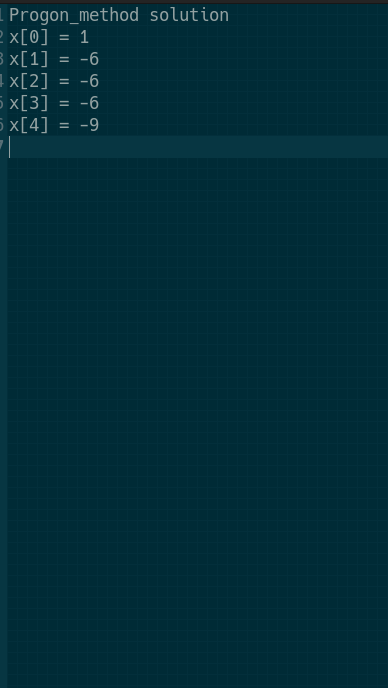
\includegraphics[width=.5\textwidth]{lab1.2}
\caption{Вывод в консоли}
\end{figure}
\pagebreak

\vfill

\subsection{Исходный код}

\lstinputlisting[title=\texttt{2.cpp}]{../stud/svoevolin/exercise_2/2.cpp}
\pagebreak